\section{Data Parallelization Common Case}

% The techniques covered above are employed during the compiler flow
% outlined in Chapter~\ref{ch:datapar} to effectively leverage data and
% task parallelism.  The coarsened StreamIt graph is converted into a
% general by employing \textsc{SynchRemove} (see
% Section~\ref{sec:synch-remove} for details).  \textsc{JudiciousFission} is
% performed on the coarsened general graph using the technique covered
% in Section~\ref{sec:levels}.  Fission of a node in the general graph
% replaces fission of a filter in the StreamIt graph (see
% Section~\ref{sec:fission-streamit}) in the process of judicious
% fission.  Conversion to the general graph with synchronization
% removal, accompanied by employing general fission, greatly reduces the
% inter-core communication requirement of the resulting mapping when
% fissing filters that peek.  Figure~\ref{fig:fission-versus} gives a
% simple example of the potential savings.

% The design of the general fission algorithm was informed by the fact
% that for most fission applications of judicious fission, a producer
% and consumer are fissed by an equal width.  This is because in most of
% our benchmarks, a level's width of task parallelism is equal to the
% width of task parallelism for it's consuming level.  In this case,
% fission on the general graph will map the bulk of communication to
% intra-core resources.  Furthermore, in the next section we demonstrate
% that the ratio of inter-core communication to total communication is
% parametrizable for this case.

To understand why general fission achieves the reduction of inter-core
communication for this case, we must remember a few properties of the
steady-state schedule of the stream graph.  For single output producer
$f$ and single input consumer $g$, where $(f,g) \in E$:

\[ M(S, f) \cdot u(W, f) = M(S,g) \cdot o(W,g) \]

\noindent When $f$ and $g$ are fissed (employing general fission) by
the same amount $P$, the above equality no longer holds across all the
fission products if $g$ peeks.  This is because the peeking of $g$ is
converted into duplication of items to the products of $g$'s fission
application.  The fission products of $g$ each consumes more items
than each fission product of $f$ produces.  However, we can make it
the case that {\it most} of the outputs of a fission product $f_i$ are
directed to $g_i$, for each $1 \le i \le P$.  When each $f_i$ and
$g_i$ are mapped to the same core, the bulk of communication is
intra-core.

\begin{figure*}[t]
\centering
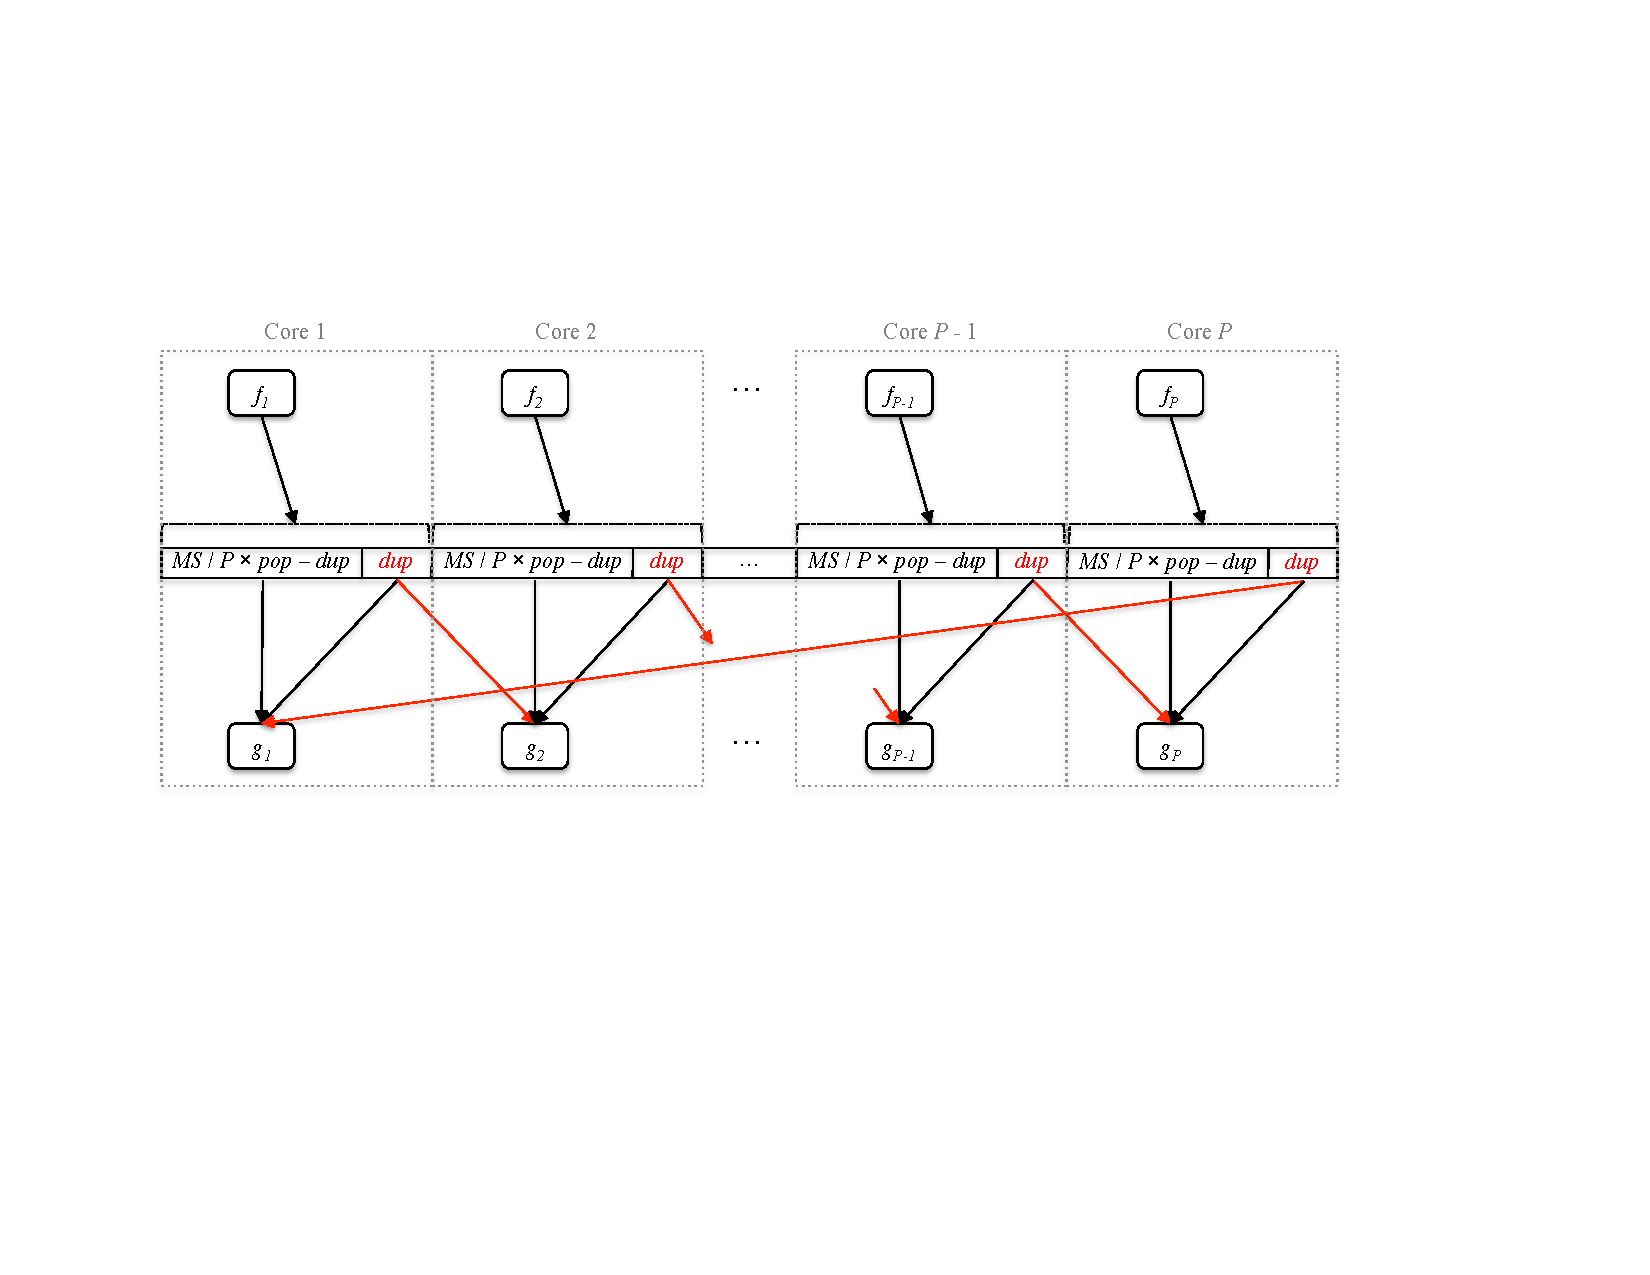
\includegraphics[width=6in]{figures/core-comm.pdf}
\caption[Communication between cores for fission of producer and
consumer.]{ Communication details for fission products of consumer $f$
  and producer $g$ each fissed by $P$.  $f$ was a single output node,
  and $g$ was a single input node.  Furthermore, $C(g) = \mt{dup}_g$.
  Each $f_i$, $g_i$ pair are mapped to the same core.
  The sizes of the buffer sections are in terms of $g$. Red arrows
  denote inter-core communication. \label{fig:core-comm}}
\end{figure*}

Figure~\ref{fig:core-comm} illustrates the details of communication
between $f$ and $g$ when each is fissed by $P$.  In the figure it is
assumed that $C(g) = \mt{dup}_g $, meaning the number of items
remaining after the initialization schedule equals the number of items
that $g$ inspected but did not pop.  Each $f_i$ produces $M(S,f)/p
\cdot u(S,f)$ items, while each $g_i$ must consume the original pop
rate multiplied by it's slice of $f$'s multiplicity plus the number of
inspected items of $g$:

\[ M(S,g)/P \cdot o(W, g) + C(g) \]

\noindent Since $M(S,g)/P \cdot o(W, g) = M(S,f)/p
\cdot u(S,f)$, the number of items each $f_i$ produces and the number
of items each $g_i$ consumes differs by $C(g)$.
As Figure~\ref{fig:core-comm} demonstrates, each $g_i$
receives $C(g)$ duplicated items from $g_{i-1}$ (with $g_1$
receiving from $f_p$).  When the fission products are assigned to
cores as given in the figure, the percentage of inter-core
communication to total communication can be reduced to:

\begin{equation}
\label{eq:min-dup}
\mt{InterCore}(g) = \frac{C(g)}{M(S,g) / P * o(W, g)}
\end{equation}

\noindent This percentage corresponds to the best case, in which a
producer and consume are fissed by the same amount and $C(g) =
\mt{dup}_g$.  This case is common in our benchmarks.

The next section covers a technique that seeks to decrease the percentage
of total communication that must be communicated inter-core.  The
technique directly decreases the number of items that are shared,
while also increasing the alignment of communication to minimize
inter-core communication.
